\chapter{Background}
%https://www.researchgate.net/figure/A-bidirectional-system-with-distributed-generation_fig2_286569839
%This section gives an overview of the conducted research work to provide a central theme for the reader of this doctoral thesis. This overview should help to understand each individual paper in the annex, representing essential parts of this doctoral thesis, in the overall context of the developed optimization methodology.

The voltage control problem has been studied for years, but it only comes under the spotlight in recent years for the increasing number of distributed resources introduced in the networks. It is important to control the voltage in an electrical power system for a regular operation of the electrical equipment, to prevent damage such as overheating of generators and motors, to reduce transmission losses and to maintain the ability of the system to last and prevent voltage collapse. \\

%https://electrical-engineering-portal.com/how-reactive-power-is-helpful-to-maintain-a-system-healthy
In particular, it is useful and needed to reduce the output of renewable generators from what they could otherwise have produced given the available resources, often referred to as the process of \textbf{curtailment}. Such generation curtailment, along with storage and transmission losses, constitute the principal sources of energy loss that could be minimised with active network management \gls{ANM} \cite{gym-anm}. \\

\noindent Controlling the voltage in an active way has many interesting properties:
\begin{itemize}
    \item It is a combination of local and global problem: the voltage at each node is influenced by the powers of all other nodes, but the impact depends on the distance between them.
    \item It is a constrained optimization problem where the constraint is to keep the voltage in a given range and the objective is to minimise the total power loss.
    \item Voltage control has a relatively large tolerance, and there are no severe consequences if the control fails to meet the requirements for short periods of time. \cite{wang2022multiagent}
    \item It is a hierarchical problem where much information is available at the top of the pyramid (distribution stations and substations) and they decrease at the base of the pyramid (houses, factories) mainly due to the absence of many sensors.
\end{itemize}

\section{Power system}
\subsection{Description of a power system}
%https://www.generatorsource.com/Articles/Generator-Info/High-Medium-and-Low-Voltage-Differences.aspx
%Power systems are facilities that produce and transport electricity to consumers. \\
Power transmission systems consist of an interconnected set of overhead lines, cables and related equipment that are used for the transfer of electricity at high voltage levels
between supply points and load points, such as customers and other electric systems. \\

In the traditional power system, electricity is produced in large, centralised power plants. The electricity is then transferred to the loads using the transmission and distribution networks. High and extra-high voltages are associated with supply transmission from the power plant. The reason for transmitting power at high and extra-high voltage levels is to increase efficiency. The lower current accompanying the high voltage transmission allows for the use of thinner, lighter-weight cables. This reduces the cost in the tower and electrical line construction. High and extra-high voltages refer to voltage magnitudes $35 kV \leq V < 220 kV$ for the high voltage and $V \geq 220 kV$ for the extra high voltage. (\emph{Symbols problem: V for voltage magnitude and V for volts?})\\
Large industrial complexes and factories that require a substantial amount of power often utilise medium supply voltages. The high voltage coming from the power plant is sent to the primary substation, this can supply step-down power to secondary substations or to single buildings. Secondary substations can have transformers to further step down the power, and they are generally located in areas that can serve one or more buildings. Medium voltages refer to voltage magnitude $1 kV \leq V < 35 kV$. \\
Then the medium supply power is step down again to a low voltage and sent to the domestic household or home appliances power supply. Low voltages refer to voltage magnitude $V < 1 kV$. \\
\begin{figure}[H]
\centering
    % 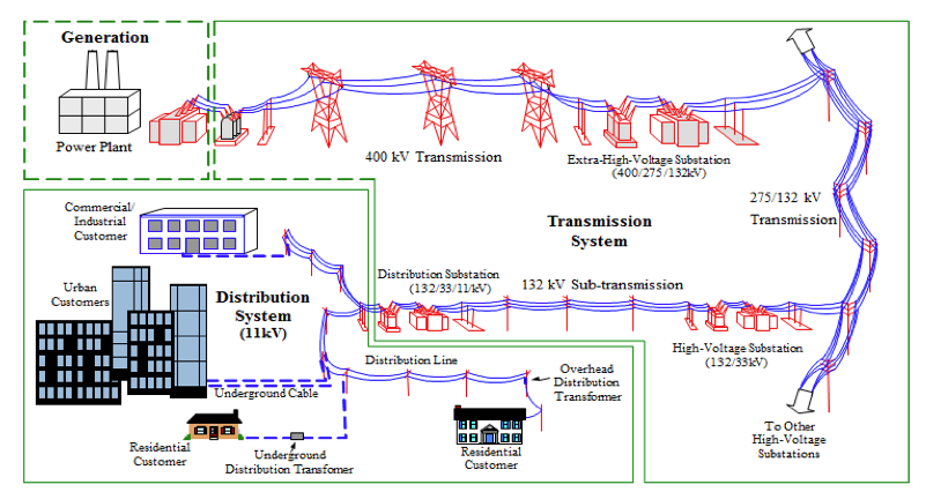
\includegraphics[width=.9\linewidth]{images/DN/HighMediumLowV.png}
    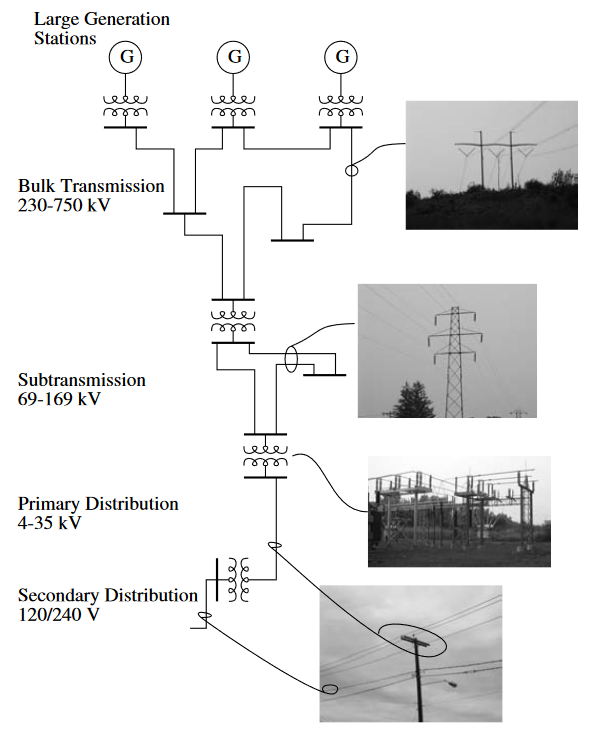
\includegraphics[width=.25\linewidth]{images/DN/DN.PNG}
\caption[Power network distribution]{Power network distribution \cite{EPD}}
% \label{fig:gym_anm_net}
\end{figure}


\noindent A power system is usually made up of the following main elements: \label{networkeledesc}
\begin{itemize}
    \item \textbf{Generator}. These produce energy, converting a form of energy into electricity. Many generators produce energy using turbines: a mass of air or water spin the generator's blades, producing electricity. This mass can be natural: hydroelectric, wind or geothermal turbines, or generated by combustion of some fuel, for example natural gas or nuclear source. \\
    There are other generators that do not need a turbine to generate electricity, for example solar panels.
    \item \textbf{Transformers}. Transformers are used to interlink systems operating at different voltages. These can increase  the voltage magnitude near a generator power plant or decrease it near the consumptions facilities. \\
    Changing the voltage magnitude allows reducing the power loss due to transportation: the power lost is given by $P=VI$, where \gls{V} is the voltage and \gls{I} is the current, so decreasing the voltage can reduce the energy loss.
    \item \textbf{Lines}. These transport the power from where energy is generated to where it is consumed. One of the main issues about transportation lines is insulation. \\
    There are different types of lines: overhead cables, they use air to insulate the bare conductors or underground cables, for these cables particular attention must be taken to insulate them from other conductors and from the earth (ground). Also, the material used must be resistant to damages, corrosion, and it must avoid that the water is being absorbed.
    \item \textbf{Switchgear}. In an electricity supply, it is necessary to disconnect equipment from the network quickly if a fault occurs to avoid damage on the elements of the network, or to disconnect some points of the network to avoid excessive losses or too high or low voltages. \\
    Switchgear is a broad term that describes a wide variety of switching devices that fulfil the need of controlling, protecting, and isolating power systems. Among these switching devices the most common are: \emph{circuit breaker}, during an electrical fault, a circuit breaker will detect the anomaly and interrupt the power flow, effectively limiting damage to the system; \emph{switch} is an electrical component that can disconnect or connect the conducting path in an electrical circuit, interrupting the electric current or diverting it from one conductor to another; \emph{recloser} similar to the circuit breaker but used in high voltage networks, these devices handle trouble temporary occurrences such as lightning, windblown tree branches or wires,
    birds, or rodents damaging the wires.
    
    \item \textbf{Loads} are electric components that consume the electric power generated by the generators. The type of loads can be divided base on the consumption in:
    \begin{itemize}
        \item[] \emph{Domestic loads}, the domestic loads mainly consist of lights, fan, refrigerator, air conditioners, mixer, grinder, heater, ovens, small pumping, motor, etc. The domestic loads consume very little power.
        \item[] \emph{Commercial loads}, the commercial loads mainly consist of lightning, fans, heating, air conditioning and many other electrical appliances used in establishments such as markets, restaurants, shops. This type of load occurs for more hours during the day as compared to the domestic load.
        \item[] \emph{Industrial loads}, the domestic loads refer from a small-scale industry, to a heavy industry. It includes all electrical loads used in industries along with the employed machinery. Industrial loads may be connected during the whole day \cite{EDNdesign}.
    \end{itemize}
    % \item Load buses where \gls{P} and \gls{Q} are specified.
    % \item Generator buses where the voltage magnitude \gls{V} and the power \gls{P} are specified.
    % \item A primary bus, an "infinite" bus, where the magnitude voltage \gls{V} is specified (normally 1 \gls{pu}) and its phase angle \gls{Vangle} is assumed to be zero as a reference angle. At this bus, both \gls{P} and \gls{Q} can be what is needed to keep the network stable. \cite{eps}
\end{itemize}

\subsection{Power flow}
\label{powerflow}
%Mathmatical formulation: https://www.engineering.iastate.edu/~jdm/ee458_2011/PowerFlowEquations.pdf
%Simple discussion: https://www.pterra.com/power-flow-analysis/power-flow-solution-techniques/
An important calculation in power system networks is to solve the optimal power flow (\gls{OPF}). \\

The power flow is essential for planning purposes: besides the calculation of electrical characteristics of the power system, power flow analysis can also help to optimize the system operating conditions and minimize the power losses.

\subsubsection{Buses}
The power flow gives information about the steady state of the entire system such as voltage, real and reactive power, line loadings and power injection.\\
Each bus is associated with four quantities: voltage magnitude \gls{V}, phase angle \gls{Vangle}, real power \gls{P} and reactive power \gls{Q}.
Depending on the quantity that have been specified, buses in the power system are classified into the following three different types:
\begin{itemize}
    \item \textbf{Slack bus}. It is taken as reference where the magnitude and phase angle of the voltage are specified. Slack bus magnitude considers 1 \gls{pu} and phase angle 0 degrees. This bus provides the additional real and reactive power to supply the transmission losses, since there are unknown until the final solution is obtained.

    \item \textbf{Load buses or PQ bus}. At these buses, the real and reactive powers are specified. The magnitude and phase angle of the bus voltage are unknown until the final solution is obtained.

    \item \textbf{Voltage controlled buses or PV bus}. At these buses, the real power and voltage magnitude are specified. The phase angles of the voltages and the reactive power are unknown until the final solution is obtained. The limits on the value of reactive power are also specified. 
\end{itemize}

\subsubsection{Solution techniques}
Solution of the power flow is based on Ohm’s Law, which is the relationship between voltages and currents. For a network, it can be expressed in matrix notation as follows:
\[
    \mathbf{I} = \mathbf{Y} \times \mathbf{V}
\]
\[
 \begin{bmatrix}
 I_1 \\ I_2 \\ \vdots  \\ I_N
 \end{bmatrix}
 = 
 \begin{bmatrix}
 Y_{1,1} & \cdots & Y_{1,N} \\
 Y_{2,1} & \cdots & Y_{2,N} \\
 \vdots & \ddots & \vdots \\
 Y_{N,1} & \cdots & Y_{N,N} \\
 \end{bmatrix}
 \times
 \begin{bmatrix}
 V_1 \\ V_2 \\ \vdots \\ V_N
 \end{bmatrix}
\]

\noindent Where:
\begin{itemize}
    \item \textbf{I} is an array of bus current injections (positive value when generation, and negative value when load)
    \item \textbf{Y} is the bus admittance matrix
    \item \textbf{V} is an array of bus voltages
\end{itemize}

The power flow formulation is based on the application of Kirchhoff’s laws to meshed electric networks. The basic concept is that the sum of all flows into each and every node should be equal to zero. The flows are in complex form, they consist of real and reactive components, or \glspl{W} and \glspl{VAR}. If there are n nodes, then there are n complex equations. The resulting system of equations is non-linear, making the calculations not easy. Solution methods are primarily iterative with the objective of reducing the sum of flows in all nodes to some acceptably small value known as the mismatch tolerance. \\

All these iterative methods and follow the same basic concept: they assume starting values for the dependent variables, primarily voltage at nominal voltage magnitude (i.e. 1 \gls{pu}) and zero phase angle; compute new values for those voltages using the nodal network equation or a numerical approximation and repeat until the convergence criteria are met.

\subsubsection{Convergence}
Convergence is the state when all nodes have met the mismatch tolerance. The main power flow solution methods are:
\begin{itemize}
    \item Gauss-Seidel method updates the     voltage one node at a time until all nodes are within the mismatch tolerance.
    
    \item Newton-Raphson method uses a first order expansion of the power flow equations to approach convergence. Generally faster than the Gauss-Seidel method and able to converge to small tolerances. However, the method is prone to the phenomenon of \textbf{divergence}, when mismatches increase instead of decrease from iteration to iteration. This occurs when the solution vector exits outside the feasible solution space at any point during the algorithm. Once outside feasible space, the solution gradient tends to further increase mismatches, leading to solutions that “blow-up” in the numerical sense. This method requires calculating the first order approximation matrix (known as the Jacobian). \\
    Several variations on the Newton-Raphson are in use, including:
        \begin{itemize}
            \item[] Fast Decoupled: separates the loosely linked real and reactive components of the power flow equations in order to speed up solution.
            \item[] Fixed Newton: does not update the first order approximation matrix every iteration to reduce computational burden.
            \item[] Non-divergent power flow: applies a reduction to the Jacobian multiplier whenever the solution appears to exit feasible space. In certain situations, this may prevent divergence, or at least stop it before blow-up.
        \end{itemize}
    \item Interior-Point Newton method forces the solution inside feasible space to avoid divergence. The interior point method uses a second order expansion of the power flow equations as a basis for its algorithm. The method is more computationally intensive than either the Gauss-Seidel or Newton-Raphson, but is less susceptible to numerical divergence.
\end{itemize}

\subsubsection{Divergence}
Divergence is the condition of the power network when the numerical solution can not be found anymore due to some possible issues:

\begin{itemize}
    \item the power system is going to “blow-up.”
    \item the power system is in voltage collapse.
    \item the power system is unstable.
    \item the initial conditions defined were bad or poor.
    \item some issues related to software or input data.
\end{itemize}

Divergence of the power flow solution has traditionally been associated with the singularity of the Jacobian matrix. Since some methods require an inverse of the Jacobian as part of its solution algorithm, singularity of the Jacobian means division by zero \cite{eps}.


\subsection{Power system reliability}
\label{sec:psr}
%https://info.ornl.gov/sites/publications/Files/Pub57467.pdf
Reliability is an important factor concerning the quality of energy supply. \\
Power reliability can be defined as the degree to which the performance of the elements in a system results in electricity being delivered to customers within accepted standards and in the desired amount \cite{MPRPQ}. \\
Reliability indices typically consider such aspects as:
\begin{itemize}
 \item the number of customers;
 \item the connected loads;
 \item the duration of the interruption measured in seconds, minutes, hours, or days;
 \item the amount of power interrupted;  
 \item and the frequency of interruptions.
\end{itemize}

These factors depend on variable such as reliability of individual items of equipment, circuit length and loading, network configuration, distribution automation, and available transfer capacity \cite{EDNdesign}. \\

For reliability purposes, it is important to know the maximum voltage that can be
transferred with transmission lines to meet the anticipated load demand. It is also important to know the levels of power through various transmission lines under certain contingency outage conditions to maintain the continuity of service. Knowledge of power flows and voltage levels under normal operating conditions are necessary in order to determine fault currents and the ensuing consequences on the stability of the system \cite{eps}. \\

%Determining power flow requires measurements of some power system conditions; utilities measure a combination of quantities such as voltage magnitude \gls{V}, real power \gls{P} and reactive power \gls{Q} of the elements connected to the network. 

\subsubsection{Reliability criteria}
\label{ssec:n1cri}
The goal of a distribution system operator (\gls{DSO}) is to ensure a reliable system. Unfortunately, a completely reliable electricity supply is not feasible to obtain since it comes at an infinite cost. So, network operators need to determine an acceptable reliability level, by balancing the costs and benefits, where acceptable reliability level means that all the elements in a network have an acceptable voltage range. \\

The European \gls{GARPUR} project (\textbf{G}enerally \textbf{A}ccepted \textbf{R}eliability \textbf{P}rinciple with \textbf{U}ncertainty modelling and through probabilistic \textbf{R}isk assessment) developed reliability management approaches and criteria. One of these criteria used by system operators is the N-1 criterion. \\

The basic principle of N-1 security in network planning states that if a component, for example a transformer or circuit, should fail or be shut down in a network operating at the maximum levels of transmission and supply, the network security must still be guaranteed. This means that the safety of the system is guaranteed and the spreading of the failure is avoided. \\

With the increasing of network complexity more than one element may fault, for this reason there exists other levels of reliability, like the N-2 criteria. In this case, even if in the network two components fail, the network security is guaranteed. \\
This N-2 criteria requires much more computational power since, the system operator must calculate what happens to the network for any combination of two fault elements. So, the problem becomes a combination problem, where the possible combination are given by: $N \choose 2$, with $N$ the number of elements in the network. \\

In general, the calculation can be extended to any generic $k$ elements, but the complexity of the problem increases with the value of $k$. Indeed, the possible combination in a N-k contingency are: $N \choose k$, with $2 < k < N$

% \section{Power system voltage managment}



